\documentclass[../main.tex]{subfiles}
%!TEX root = ./analysisConnector.tex
\graphicspath {{../}}

\begin{document}

\subsection{Connection To Keel} \label{connector}
\begin{figure}[H]
	\centering
	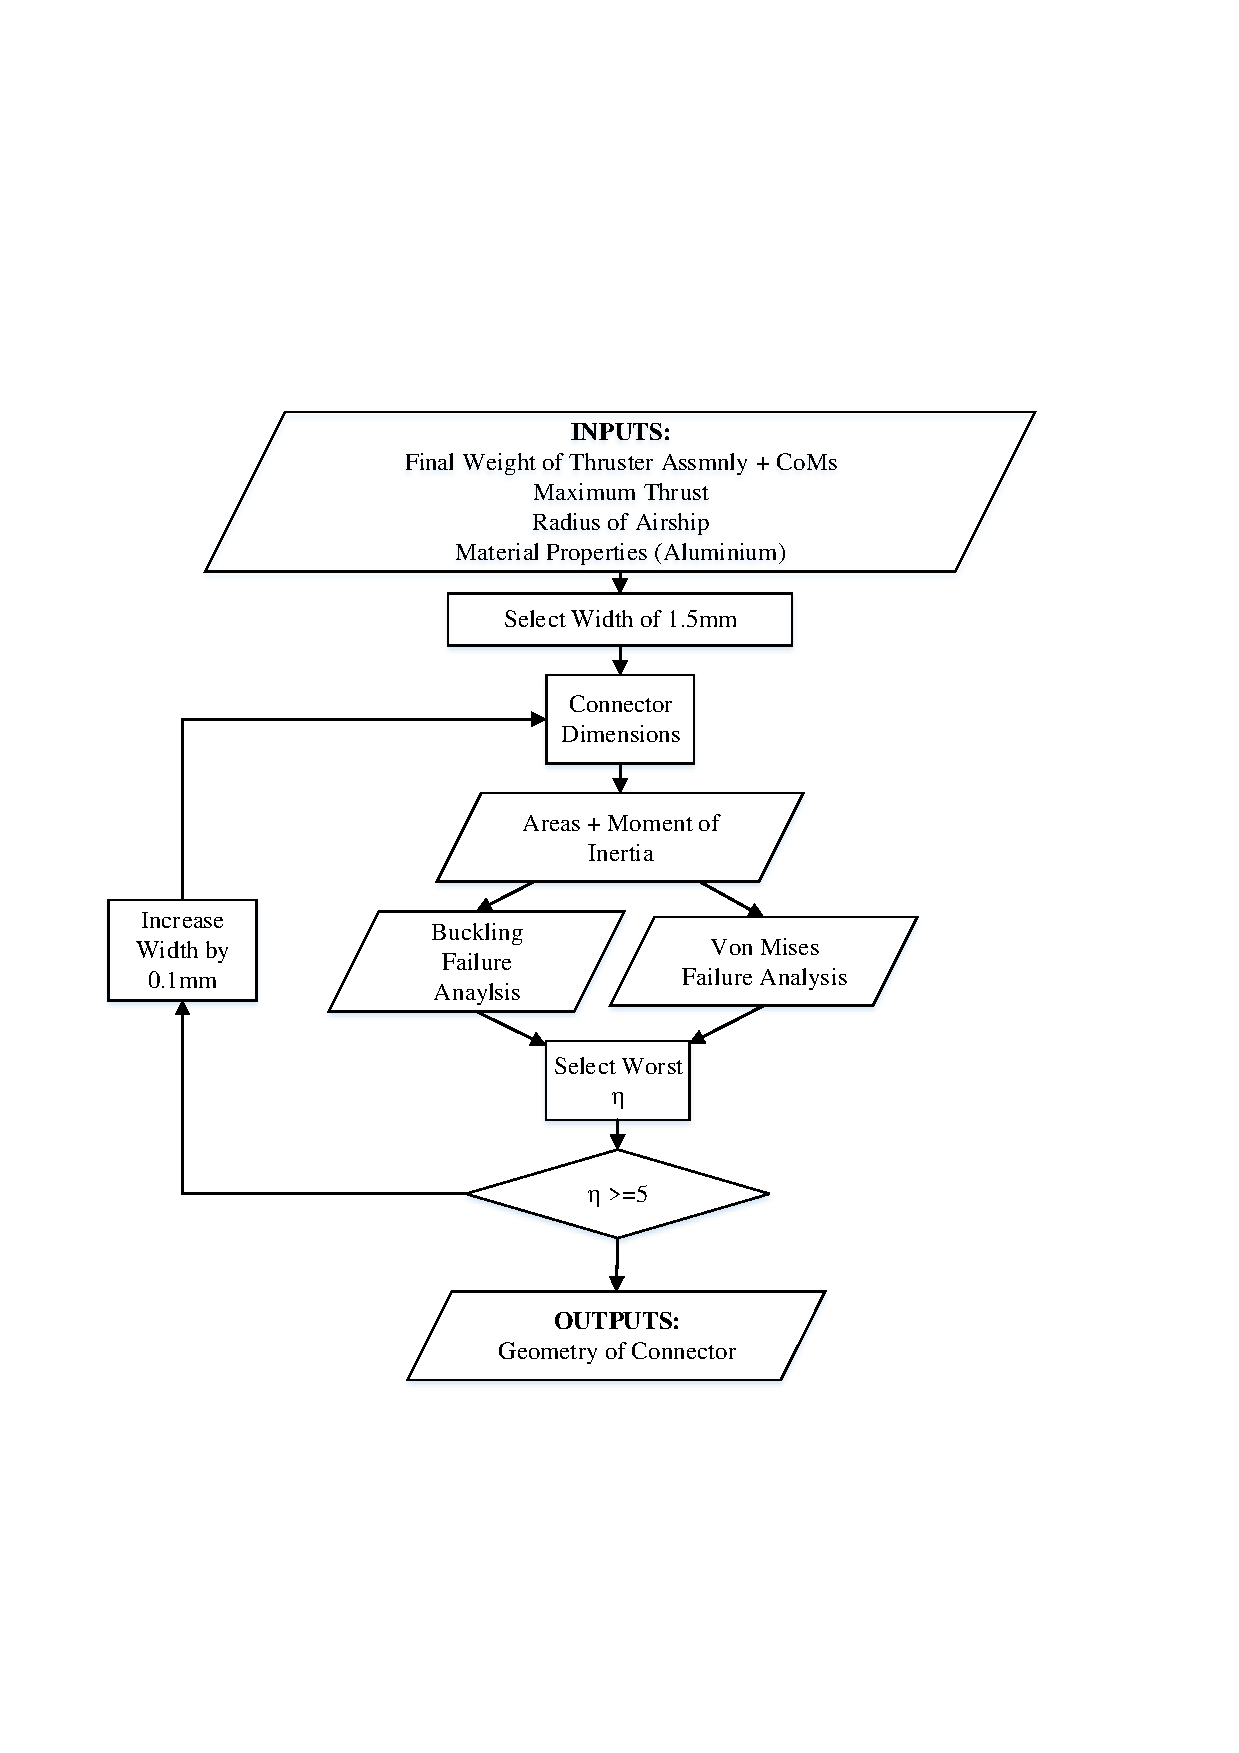
\includegraphics[width=.9\linewidth]{img/paramaterization/connector.pdf}
	\caption{Parametrization Outline for the Thruster Arm Connector}
	\label{fig:connectorParametrization}
\end{figure}

This section analyses the thruster arms connection to the keel. It uses a rectangular piece that attaches to the bottom of the arm and the piece used for connecting the sections of keel together. The analysis outputs the geometry of the connector piece such that it meets the safety factor of 5 assigned to the component. The inputs required in order to perform the analysis include the final weight of thruster assembly and its centre of mass data, the radius of the thruster arms and the material properties aluminium 6061 \cite{AlProperties}. \\

The first analysis relates to the loading scenario described in Section \ref{loadingScenarios}, shown specifically in Figure \ref{fig:scenario1}. In this scenario, the connector holds the weight and thrust forces in the x-direction. The assumption is that the two failures can occur from buckling and bending of the piece. The main focus of analysis is the bending of the piece. A free body diagram of the top of the connector can be seen in Figure \ref{fig:armConnector}. 

\begin{figure}[H]
	\centering
	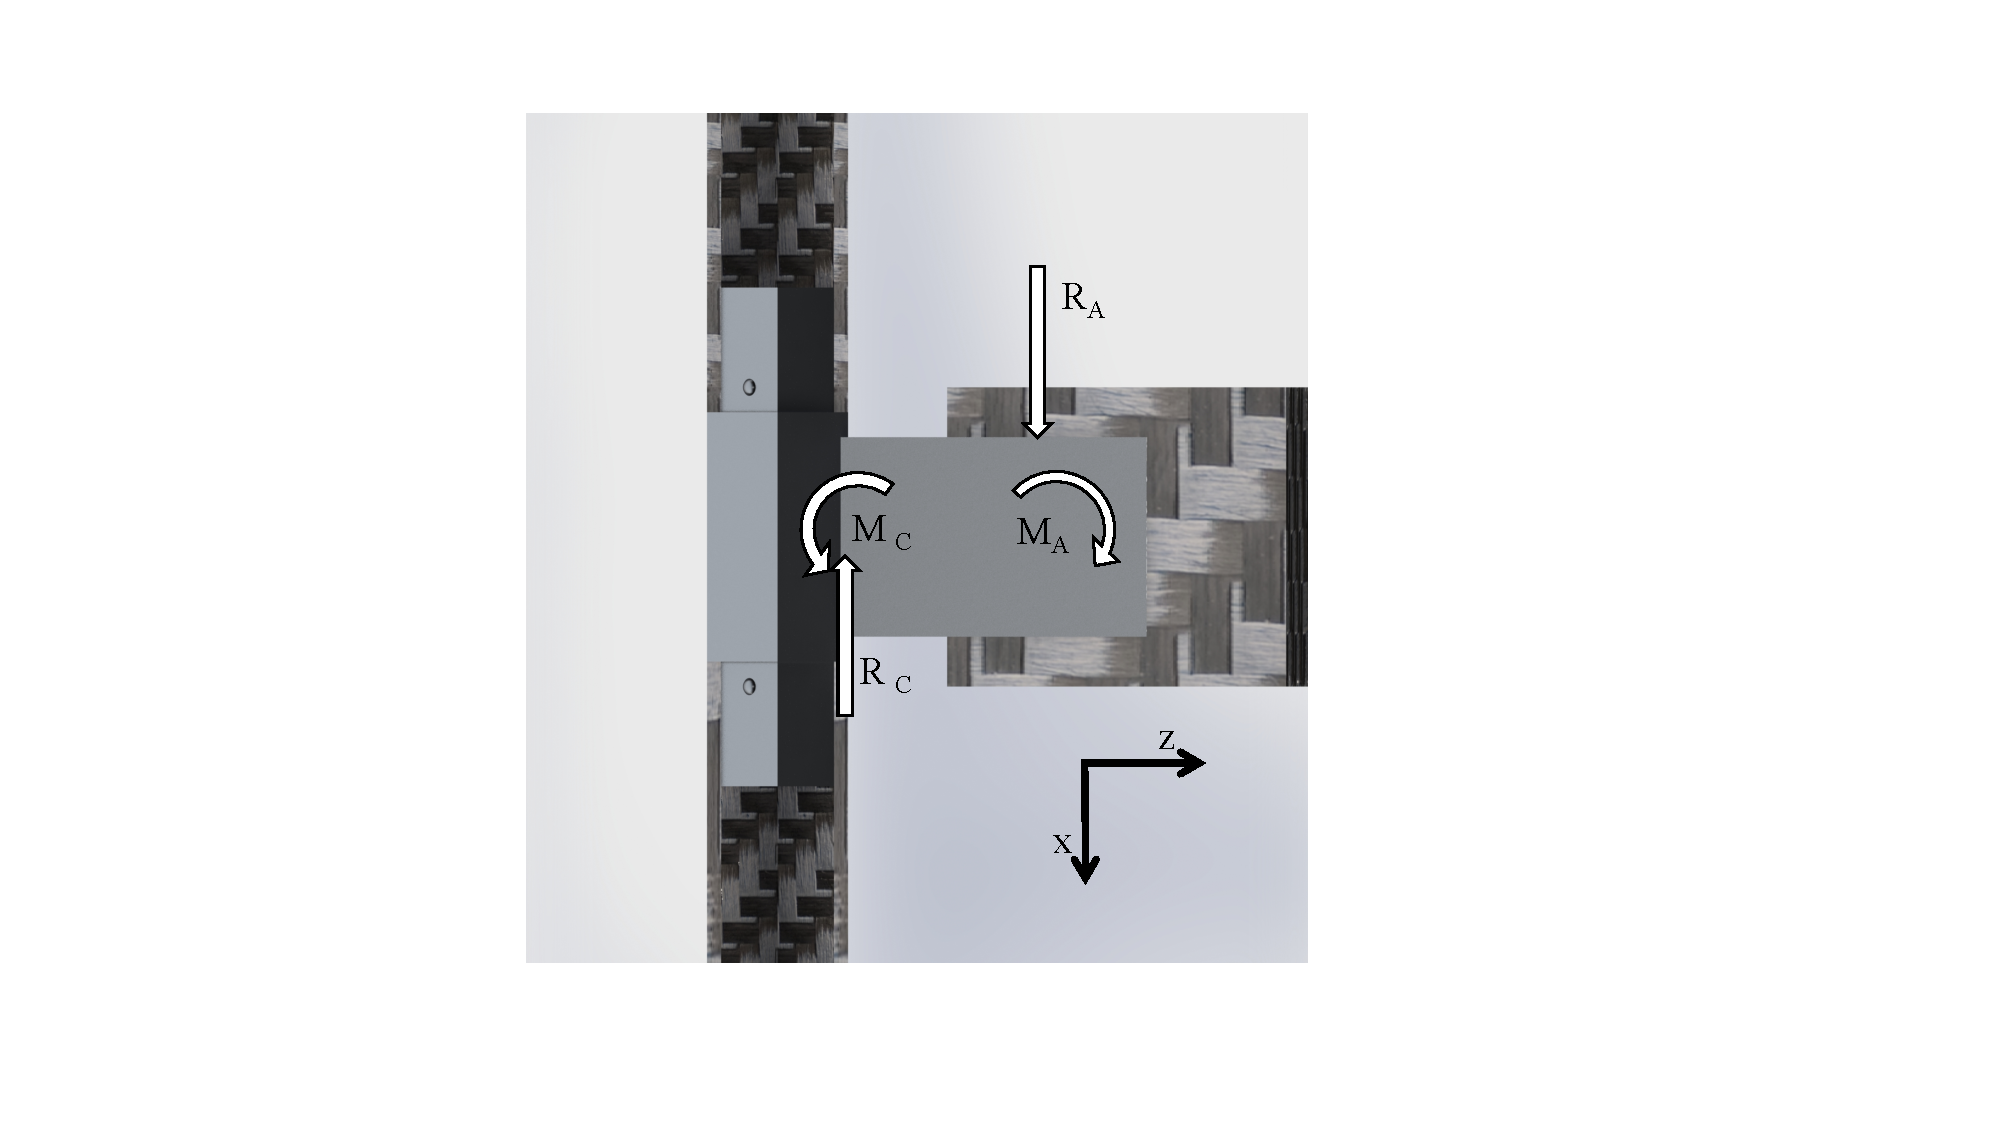
\includegraphics[page={1}, width=.7\linewidth]{img/analysis/arm/armConnector.pdf}
	\caption{Free Body of the Connector Piece in the Worst Case Scenario}
	\label{fig:armConnector}
\end{figure}


The analysis uses the reaction forces generated by the arm in this scenario. The loading is very simple in this case, with the reaction force at $C$ equalling the input force, and the reaction moment resisting the moment and the force generated moment. To resolve these forces, forceSolver \ref{code:forceSolver} code is used. The stress in the connector has multiple plane bending in some cases, and is represented in Equation \ref{eqn:connectorztress}, where the $M$s are the reaction moments and the $I$s are the moments of inertia across the cross section. The $c$s are the distance from the neutral axis to the point of analysis, $Fz$ is the force in the $z$ direction, and $A$ is the area of the cross-section.

\begin{equation}
\label{eqn:connectorztress}
\sigma_{z}=  \underbrace{\frac{M_{x}c_y}{I_x}}_\text{Bending moment stress about x} + \underbrace{\frac{M_{y}c_x}{I_y}}_\text{Bending moment stress about z} + \underbrace{\frac{F_z}{A}}_\text{Axial stress} 
\end{equation}

In the worst case loading scenario as shown in Figure \ref{fig:armConnector}, both $F_y$ and $M_z$ are zero. In addition to the planar stress in z it is also possible to have torsional shear in the xy plane. This is described by Equation \ref{eqn:armtorsionShear} from {(Shigley's Machine Design \cite[102]{shigley})}. This will only occur if there is differential steering on the arms and will not be included in the analysis of this scenario.

\begin{equation} \label{eqn:armtorsionShear}
\tau_{xy} = \dfrac{M_{z}}{wt^2}(3+\frac{1.8t}{w})
\end{equation}

Next, the analysis takes both the planar and shear stresses and converts them to principle stresses (as shown in Appendix \ref{appendix:cauchy}). These principle stresses are then used to determine the safety factor by Von Mises Theory \cite[221]{shigley}.

\begin{equation}
\eta = \dfrac{S_{ut}}{\sigma _a} \Rightarrow 5 \geq \dfrac{S_{ut}}{\sigma _a}
\end{equation}

A safety factor of five was chosen because the likelihood of failure was evaluated as being high, and the component is critical to operation of the airship.

\paragraph*{Buckling}

Another type of failure which could occur is buckling. Buckling could occur at the top part of the connector. The loading for this scenario has all the forces acting downwards in the z-direction. This can be seen  in Figure \ref{fig:armConnectorBuck}.

\begin{figure}[H]
	\centering
	\includegraphics[page={2}, width=.8\linewidth]{img/analysis/arm/armConnector.pdf}
	\caption{Free Body for Buckling of the Connector}
	\label{fig:armConnectorBuck}
\end{figure}

The buckling is calculated using Euler's critical load \cite[178]{shigley}. Where $C$ is an end constant taken as $1.2$ for this case, $E$ is the modulus of elasticity, $l$ is the height shown in Figure \ref{fig:armConnectorBuck}, and $I_z$ is calculated using: 

\begin{equation} \label{eqn:EulersCriticalForce}
P_{cr} = \frac{C\pi^2EI_z}{l^2}
\end{equation}

\begin{equation}
I_z = \frac{b^3l}{12}
\end{equation}
Plugging these values into Equation \ref{eqn:EulersCriticalForce}:
\begin{equation}
P_{cr} = \frac{(1.2)\pi^2Eb^3}{12l}
\end{equation}

The safety factor is calculated using the force applied and the critical force (Equation \ref{eqn:EulersCriticalForce}):
\begin{equation}
\eta = \frac{P_{cr}}{F_{Rz}}
\end{equation}

\paragraph*{Sample Calculations}
$M_y$ and $F_{Rz}$ values taken from the MATLAB Force Solver.
\paragraph*{Von Mises}
$$\sigma_{z}={\frac{M_{x}c_y}{I_x}}+{\frac{M_{y}c_x}{I_y}}+{\frac{F_z}{A}}=0+\frac{(17.2196N\cdot{}m)(0.0200m)}{8.000\cdot{}10^{-9}mm^4}+0 = 43.049MPa$$
$$\eta = \dfrac{S_{ut}}{\sigma _a} = \dfrac{310MPa}{43.049MPa}=7.2$$
\paragraph*{Buckling}
$$P_{cr} = \frac{(1.2)\pi^2Eb^3}{12l}=\frac{(1.2)\pi^2(68.9\cdot{}10^9Pa)(0.0015m)^3}{12(0.0330m)}=6954.71N$$
$$\eta = \frac{P_{cr}}{F_{Rz}} = \frac{6954.71N}{29.9623N} = 232$$

\end{document}